\section{Background}

\subsection{Scalar output Gaussian Process Regression}

Given training set $D = \{X, \bm{y}\}$ where $X = \{\bm{x}_1,~\dots~\bm{x}_N\}$, and $\bm{y} = \{y_1,~\dots~y_N\}$, we assume the target value $y$ is generated
by a latent function $f(\bm{x})$ such with addictive noise $\epsilon \sim N(0, \sigma_n^2)$ such that
\begin{equation}
    \label{eq:yf}
    y_i = f(\bm{x}_i) + \epsilon_i.
\end{equation}
We use Gaussian process (GP)\cite{GPML} to learn the latent function $f(\bm{x})$, a Gaussian process model defines a prior over $f(\bm{x})$. GP is fully characterized by a mean function $m(\bm{x})$ and a covariance function $k(\bm{x}, \bm{y})$. For the training set $D$, the latent function values $\bm{f} = (f(\bm{x}_1),~\dots~f(\bm{x}_N))^T$ follow a joint Gaussian distribution $\bm{f} \sim N(\bm{m}, K)$ where $\bm{m} = (m(\bm{x}_1),~\dots~,m(\bm{x}_N))^T$ is the mean vector, and $K_{ij} = k(\bm{x}_i, \bm{x}_j)$ is the covariance matrix. The mean function $m(\bm{x})$ can be any function, while the kernel function $k(\bm{x}, \bm{y})$ has to make sure that the covariance matrix is a symmetric positive definite (SPD) matrix. In this paper, we fix $m(\bm{x}) = 0$.

Given a new input $\bm{x}_*$, GP predicts the distribution of the output $y \sim N(\mu(\bm{x}_*), \sigma^2(\bm{x}_*))$, the $\mu(\bm{x}_*)$ and $\sigma^2(\bm{x}_*)$ are given by

\begin{equation}
    \left\{
        \begin{array}{lll}
            \mu(\bm{x}_*)      &=& k(\bm{x}_*, X) (K + \sigma_n^2 I)^{-1} \bm{y} \\
            \sigma^2(\bm{x}_*) &=& \sigma_n^2 + k(\bm{x}_*, \bm{x}_*) - k(\bm{x}_*, X) (K + \sigma_n^2 I)^{-1} k(X, \bm{x}_*) 
        \end{array}
    \right.
    \label{eq:GPRPred}
\end{equation}

where $k(\bm{x}_*, X) = (k(\bm{x}_*, \bm{x}_1),~\dots~,k(\bm{x}_*, \bm{x}_N))$ and $k(X, \bm{x}_*) = k(\bm{x}_*, X)^T$. In \eqref{eq:GPRPred}, the $\mu(\bm{x}_*)$ and $\sigma^2(\bm{x}_*)$ and be viewed as the prediction and the uncertainty measure.

There are usually some hyperparameters for a GP model, including the noise level $\sigma_n$ and hyperparameters for the kernel functions. For example, the squared exponential kernel is a commonly used kernel in GP regression, the kernel function is defined as

\begin{equation}
    \label{eq:GaussianCovarianceFunction}
    k(\bm{x}_i, \bm{x}_j) = \sigma_f^2 \exp\Big(-\frac{1}{2}(\bm{x}_i - \bm{x}_j)^T\Lambda^{-1}(\bm{x}_i - \bm{x}_j)\Big),
\end{equation}
where $\Lambda = \mathrm{diag}(l_1, \dots, l_d)$ is a diagonal matrix and $l_i$ denotes the length scale of the $i$-th dimension, $\sigma_f$ and $\Lambda$ are the hyperparameters for the kernel. Denote $\bm{\theta}$ as the vector of hyperparameters, the hyperparameters can be learnt via maximum likelihood estimation (MLE) by maximizing the following likelihood function

\begin{equation}
    \log p(\bm{y} | X, \bm{\theta}) = -\frac{1}{2}(\bm{y}^T K_{\bm{\theta}}^{-1} \bm{y} + \log |K_{\theta}| + N \log(2 \pi))
\end{equation}

Where $K_{\bm{\theta}}$ is the covariance matrix of the training input calculated by the kernel function. 

\subsection{NN-GP}


\begin{equation}
    f(\bm{x}) = \bm{w}^T \phi(\bm{x})
\end{equation}

\begin{equation}
    \bm{w} \sim N(0, \Sigma_p)
\end{equation}

\begin{equation}
    k(\bm{x}, \bm{y}) = \phi(x)^T \Sigma_p \phi(y)
\end{equation}

\begin{equation}
    \Sigma_p = \mathrm{diag}(\frac{\sigma_p^2}{M})
\end{equation}

\begin{equation}
    \left\{
        \begin{array}{lll}
            \mu(\bm{x})      &=& \phi(x)^T A^{-1} \Phi \bm{y} \\
            \sigma^2(\bm{x}) &=& \sigma_n^2 + \sigma_n^2 \phi(\bm{x})^T A^{-1} \phi(\bm{x})
        \end{array}
    \right.
\end{equation}

\begin{equation}
\end{equation}

\begin{equation}
\end{equation}

In (IEEE2010), the author propose to use a neural network with one hidden layer as the feature map $\phi(\bm{x})$, in (IJCAI2016), the single hidden layer is extended to multiple layers, a similar work is (DNGO), where bayesian linear regression is performed on the last layer. 

\begin{figure}[!htb]
    \centering
    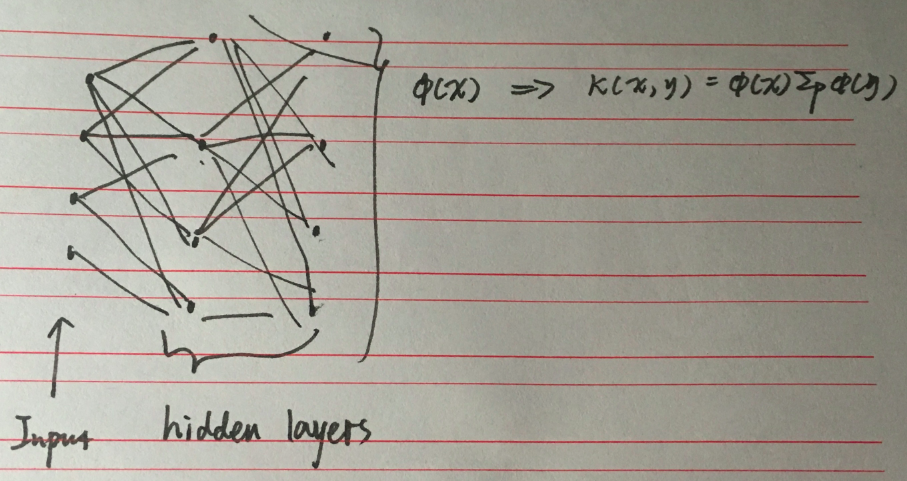
\includegraphics[width=\columnwidth]{./img/NN-GP.png}
    \caption{Architechure of the Gaussian process model with kernel characterized by deep neural network}
\end{figure}

\paragraph{Deep ensemble}

\begin{equation}
    \left\{
        \begin{array}{lll}
            \mu_*(\bm{x})      &=& \frac{1}{K} \sum_k \mu_k(\bm{x}) \\
            \sigma_*^2(\bm{x}) &=& \frac{1}{K} \sum_k (\mu_k^2(\bm{x}) + \sigma_k^2(\bm{x})) - \mu_*^2(\bm{x})
        \end{array}
    \right.
\end{equation}

In (NIPS2017DeepMind), ...
